\section{The ladder \protect
\includegraphics[height=1em]{figs/ladder.png}: Agent improvement with AutoLibra}

AutoLibra can additonally be employed to directly improve agent performance by using extracted metrics to guide targeted modifications to the agent's code, using a human-in-the-loop or another LLM as the editor.

As a demonstration of AutoLibra's capabilities, we present a case study where we use AutoLibra to improve the performance of an agent on baba-is-ai, a highly challenging agentic reasoning task based on the Baba Is You video game. We demonstrate that AutoLibra induces fine-grained, orthogonal [non-redundant], and human-interpretable metrics that have high coverage of the agent's behavior, and show the utility of these metrics in guiding targeted modifications to the agent's to improve its performance and efficiency. We further demonstrate that an agent improved by metrics extracted from AutoLibra outperforms a baseline agent on the task in environment score and trajectory performance, and that the improvements realized by AutoLibra are generalizable to unseen Baba Is You levels and arbitrary LLMs.

\subsection{AutoLibra provides optimization targets for agent prompt engineering}
\label{sec:baba-is-ai}
Baba Is You is a puzzle game in which the player controls a character that can modify the rules of the game by pushing blocks containing words that define the game's rules. Words can be combined to form sentences that define the properties of objects in the game, such as "Baba is You" or "Flag is Win". The goal of the game is to reach a win condition, such as touching a flag, by manipulating the rules of the game to create new win conditions, modify the properties of objects, or change the behavior of the player character.

The game is highly challenging and requires the player to think creatively and reason causally about the game's rules in order to solve the puzzles. This makes Baba Is You an ideal testbed for evaluating the performance of reinforcement learning agents on agentic reasoning tasks; we employ the baba-is-ai environment, a simplified version of Baba Is You \cite{cloos2024babaaibreakrules, paglieri2024balrog} as our testing implementation. Observations of the environment are supplied to the agent in text form, and the agent interacts with the environment by issuing commands in the form of text strings that move the active character.

[Insert figure of baba-is-ai environment]

\subsection{AutoLibra for baba-is-ai improvement}

In performing iterative agent improvement with AutoLibra, a full cycle of the AutoLibra pipeline is considered a full turn, the pseudocode for which is shown in Algorithm 1. One unmodified agent is used as a baseline for comparison (Turn 0), and three complete turns of iterative agent improvement with AutoLibra are performed (Turn 1, 2, 3), for a total of four turns. Six representative tasks for baba-is-ai are used in iterative metric improvement, with the remainder held out for evaluation. The agent is evaluated on the baba-is-ai environment and any changes to the agent code at the beginning of each turn, and the environment score, trajectory performance, and other metrics are recorded at the end of each turn. GPT-4o-241120 is used as the agent model.


\begin{algorithm}
    \caption{Pseudocode for iterative agent improvement with AutoLibra}
    \begin{algorithmic}[1]
    \For{$i$ in range($n\_turns$)}
        \For{$task$ in $selected\_tasks$}
            \State $traj_i, eval\_score_i += agent.play(task, prompt)$
            \State $annotations_i += editor.annotate(traj_i)$
        \EndFor
        \State $metrics_i = AutoLibra.extract_metrics(traj_i, annotations_i)$
        \State $traj\_scores_i = AutoLibra.llm_eval(metrics_i, traj_i)$
        \State $curr\_scores = eval\_score_i$
        \While {$curr\_scores <= eval\_score_i$}
            \State $prompt = updated\_prompt_k$
            \For{$task$ in $selected\_tasks$}
                \State $\_, curr_scores = agent.play(task, prompt)$
            \EndFor
        \EndWhile
    \EndFor

    \end{algorithmic}
\end{algorithm}

\begin{wraptable}[19]{r}{0.60\textwidth} % 'r' for right, adjust the width as needed
\centering
\small
\vspace{-30pt}
\begin{tabular}{ccl}
\toprule
\multicolumn{1}{c}{Emoji}& 
\multicolumn{1}{c}{It.} & 
\multicolumn{1}{l}{Metric} \\
\midrule
\rowcolor{gray!10} 
\includegraphics[scale=0.07]{figs/emojis/emoji_1.png} & 0 & Win Condition Recognition \\
\midrule
\rowcolor{gray!10} 
\includegraphics[scale=0.07]{figs/emojis/emoji_2.png} & 0 & Rule Modification \\
\midrule
\rowcolor{gray!10} 
\includegraphics[scale=0.07]{figs/emojis/emoji_3.png} & 0 & Direct Navigation Efficiency \\
\midrule
\rowcolor{gray!10} 
\includegraphics[scale=0.07]{figs/emojis/emoji_4.png} & 0 & Context-Sensitive Decision Making \\
\midrule
\rowcolor{gray!30} 
\includegraphics[scale=0.07]{figs/emojis/emoji_5.png} & 1 & Win Rule Construction \\
\midrule
\rowcolor{gray!30} 
\includegraphics[scale=0.07]{figs/emojis/emoji_6.png} & 1 & Selective Interaction With Relevant Objects  \\
\midrule
\rowcolor{gray!30} 
\includegraphics[scale=0.07]{figs/emojis/emoji_7.png} & 1 & Rule Manipulation and Execution  \\
\midrule
\rowcolor{gray!60} 
\includegraphics[scale=0.07]{figs/emojis/emoji_8.png} & 2 & Subtask Coordination \\
\midrule
\rowcolor{gray!90} 
\includegraphics[scale=0.07]{figs/emojis/emoji_9.png} & 3 & Immovable Interaction \\
\bottomrule
\end{tabular}
\caption{Metrics and Turn of Induction \newline for Baba-Is-AI}
\label{tab:metrics}
\end{wraptable}\label{tab:metrics}
% Function to generate color based on percentage value
\newcommand{\cellcolorpercent}[1]{%
  \ifdim #1 pt < 10 pt \cellcolor{red!90}%
  \else\ifdim #1 pt < 20 pt \cellcolor{red!80}%
  \else\ifdim #1 pt < 30 pt \cellcolor{red!70}%
  \else\ifdim #1 pt < 40 pt \cellcolor{red!60}%
  \else\ifdim #1 pt < 50 pt \cellcolor{red!50}%
  \else\ifdim #1 pt < 60 pt \cellcolor{yellow!40}%
  \else\ifdim #1 pt < 70 pt \cellcolor{yellow!30}%
  \else\ifdim #1 pt < 80 pt \cellcolor{green!30}%
  \else\ifdim #1 pt < 90 pt \cellcolor{green!50}%
  \else\ifdim #1 pt < 100 pt \cellcolor{green!70}%
  \else\cellcolor{green!90}%
  \fi\fi\fi\fi\fi\fi\fi\fi\fi\fi\fi\fi
}

\begin{document}

\begin{table}[ht]
\centering
\begin{tabular}{|>{\arraybackslash}p{1cm}|c|c|c|c|}
\hline
\rowcolor[HTML]{C0C0C0} 
\textbf{Turn} & \textbf{0} & \textbf{1} & \textbf{2} & \textbf{3} \\ \hline

\includegraphics[scale=0.07]{figs/emojis/emoji_1.png} & \cellcolorpercent{27.78} \textbf{27.78\%} & \cellcolorpercent{50.00} \textbf{50.00\%} & \cellcolorpercent{88.89} \textbf{88.89\%} & \cellcolorpercent{94.44} \textbf{94.44\%} \\ \hline

\includegraphics[scale=0.07]{figs/emojis/emoji_2.png}& \cellcolorpercent{5.56} \textbf{5.56\%} & \cellcolorpercent{11.11} \textbf{11.11\%} & \cellcolorpercent{27.78} \textbf{27.78\%} & \cellcolorpercent{44.44} \textbf{44.44\%} \\ \hline

\includegraphics[scale=0.07]{figs/emojis/emoji_3.png} & \cellcolorpercent{5.56} \textbf{5.56\%} & \cellcolorpercent{12.50} \textbf{12.50\%} & \cellcolorpercent{12.50} \textbf{12.50\%} & \cellcolorpercent{44.44} \textbf{44.44\%} \\ \hline

\includegraphics[scale=0.07]{figs/emojis/emoji_4.png} & \cellcolorpercent{11.11} \textbf{11.11\%} & \cellcolorpercent{12.50} \textbf{12.50\%} & \cellcolorpercent{12.50} \textbf{12.50\%} & \cellcolorpercent{38.89} \textbf{38.89\%} \\ \hline

\includegraphics[scale=0.07]{figs/emojis/emoji_5.png} & - & \cellcolorpercent{0.00} \textbf{0.00\%} & \cellcolorpercent{0.00} \textbf{0.00\%} & \cellcolorpercent{5.56} \textbf{5.56\%} \\ \hline

\includegraphics[scale=0.07]{figs/emojis/emoji_6.png} & - & \cellcolorpercent{27.78} \textbf{27.78\%} & \cellcolorpercent{44.44} \textbf{44.44\%} & \cellcolorpercent{88.89} \textbf{88.89\%} \\ \hline

\includegraphics[scale=0.07]{figs/emojis/emoji_7.png} & - & \cellcolorpercent{5.56} \textbf{5.56\%} & \cellcolorpercent{27.78} \textbf{27.78\%} & \cellcolorpercent{33.33} \textbf{33.33\%} \\ \hline

\includegraphics[scale=0.07]{figs/emojis/emoji_8.png} & - & - & \cellcolorpercent{11.11} \textbf{11.11\%} & \cellcolorpercent{33.33} \textbf{33.33\%} \\ \hline

\includegraphics[scale=0.07]{figs/emojis/emoji_9.png} & - & - & - & \cellcolorpercent{66.67} \textbf{66.67\%} \\ \hline 
Cov. & \textbf{65\%} & \textbf{83\%} & \textbf{85\%} & \textbf{92\%} \\ \hline
Red. & \textbf{58\%} & \textbf{59\%} & \textbf{47\%} & \textbf{59\%} \\ \hline
\end{tabular}
\caption{Metric Performance for baba-is-ai AutoLibra Turns 0-3}
\end{table}
\label{tab:metric_perf}
\renewcommand{\arraystretch}{1.5} 
\begin{table}[h!]

\centering
\begin{tabular}{|>{\raggedright\arraybackslash}p{6cm}|c|c|c|c|}
\hline
\textbf{Turn} & \textbf{0} & \textbf{1} & \textbf{2} & \textbf{3} \\
\hline
\textbf{Babaisai Score GPT-4o} & 0.30 & 0.40 & 0.43 & 0.55 \\
\hline
\textbf{Babaisai Score Claude 3.5 Sonnet} & 0.35 & 0.40 & 0.45 & 0.55 \\
\hline
\textbf{Average Env. Steps} & 79 & 63 & 60 & 51 \\
\hline
\end{tabular}
\caption{Babaisai Scores and Average Environment Steps}
\end{table}\label{tab:heldout}

\subsection{Results}

The induced metrics and the agent's per-task performance are shown in Table \ref{tab:metrics}, Table \ref{tab:metric_perf}, respectively. A significant improvement in the agent's is observed from Turn 0 to Turn 3, with the agent achieving a both higher environment score and trajectory performance on the held-out tasks compared to the baseline agent. Significantly, the agent's performance on specific metrics increased correspondingly to code changes targeting those metrics, demonstrating the utility of AutoLibra for fine-grained agent improvement. This is discussed in more detail in the following sections.

\subsubsection{Extracted Metrics and Improvements}
The metrics induced by AutoLibra (Table \ref{tab:metrics}) capture the behavior of the agent effectively, with coverage increasing from 65\% at Turn 0 to 92\% at Turn 3 and a low mean redundancy of 56\%. Notably, earlier metrics were found to describe higher-level behaviors than later metrics, reflective of the more complex behaviors that the agent demonstrated in later turns, as well as the compositionality of induced metrics. Code changes were selected to specifically target given metrics, and as seen in Figure \ref{fig:autolibra-training}, the agent's performance on the targeted metric improved significantly in the turn following the code change. This demonstrates the utility of AutoLibra for fine-grained agent improvement, as well as the human interpretability of the induced metrics.

\textbf{Turn 0}
The agent behavior is stochastic and inconsistent, with no clear strategy or goal. Any progress in the environment is the consequence of a random walk. 
\texttt{Win Condition Recognition} 
\includegraphics[scale=0.07]{figs/emojis/emoji_1.png} was identified as a prerequisite to all other metrics induced in this turn, as progress in the environment is impossible without recognizing the win condition, and was therefore targeted for improvement. Improvements took the form of few-shot prompting, by supplying an example of observations and the corresponding win condition and subtasks, and guidance on subtask-level planning, by mapping specific environmental observations to actions that would progress the agent towards the win condition.
\newline
\textbf{Turn 1}
An increase in 
\includegraphics[scale=0.07]{figs/emojis/emoji_1.png} performance of 22\% was observed between Turn 0 and Turn 1, indicating that the code changes were effective in improving the agent's ability to recognize the win condition. A slight but statistically insignificant increase was observed for the other metrics induced in Turn 0, but the agent's overall baba-is-ai environment score increased by 10\%, indicating that 
\includegraphics[scale=0.07]{figs/emojis/emoji_1.png} was correctly identified by AutoLibra as a key bottleneck to the agent's performance in the environment.

The agent now targets specific blocks and objects instead of moving randomly, but gets stuck in loops and on immovable objects, and is unable to consistently complete multi-step tasks.

Based on the metrics induced in Turn 1, several changes to the agent code were implemented:
\begin{itemize}
    \item Augmentation of existing subtask-level planning guidance with low-level position instructions, targeting improvement of \texttt{Rule Modification for Obstacle Management} 
\includegraphics[scale=0.07]{figs/emojis/emoji_2.png} and \texttt{Direct Navigation Efficiency} 
\includegraphics[scale=0.07]{figs/emojis/emoji_3.png}
    \item Meta-prompting \cite{Suzgun_Kalai_2024} by providing subtask identification heuristic, targeting improvement of \texttt{Selective Interaction with Relevant Objects} 
\includegraphics[scale=0.07]{figs/emojis/emoji_6.png} and \texttt{Context-Sensitive Decision Making} 
\includegraphics[scale=0.07]{figs/emojis/emoji_4.png}
    \item Augmentation of single-shot example with movement instructions, targeting improvement of \texttt{Rule Manipulation and Execution} 
\includegraphics[scale=0.07]{figs/emojis/emoji_7.png}
\end{itemize}


\textbf{Turn 2}
Substantial improvements in 
\includegraphics[scale=0.07]{figs/emojis/emoji_1.png} were observed due to more detailed single-shot examples and reasoning templates, and the corresponding increase in other metrics supports idea that 
\includegraphics[scale=0.07]{figs/emojis/emoji_1.png} is a key bottleneck to the agent's performance. We further observed a significant increase in 
\includegraphics[scale=0.07]{figs/emojis/emoji_2.png} and 
\includegraphics[scale=0.07]{figs/emojis/emoji_7.png}, indicating that the changes targeting these metrics were effective in improving the agent's reasoning performance and consequent avoidance of irrelevant objects. \texttt{Subtask Identification} 
\includegraphics[scale=0.07]{figs/emojis/emoji_5.png} saw no significant improvement, as the agent still misunderstands map directions and confuses rule blocks with objects. 

Qualitatively, the agent now recognizes when wall rules need to be broken and breaks them, but still cannot assemble rules to win, as it gets stuck on immovable blocks and walls and does not understand where rule blocks need to be placed to form a win condition.

Based on the metrics induced in Turn 2, several changes to the agent code were implemented:
\begin{itemize}
    \item Formatting observations as absolute position (as opposed to relative steps from the agent), and listing of immovable/movable blocks to improve \texttt{Direct Navigation Efficiency} 
\includegraphics[scale=0.07]{figs/emojis/emoji_3.png}
    \item Chain-of-thought reasoning to assemble subtask completion agenda based on turn-to-turn observations, targeting improvement of \texttt{Subtask Coordination and Overall Task Planning} 
\includegraphics[scale=0.07]{figs/emojis/emoji_8.png}
    \item Augmentation of single-shot example to few-shot example with reasoning templates, targeting improvement of \texttt{Rule Manipulation and Execution} 
\includegraphics[scale=0.07]{figs/emojis/emoji_7.png}
    \item Explicit instructions on navigation to avoid block collisions and assembly of rules, including movement templates, targeting improvement of \texttt{Rule Manipulation and Execution} 
\includegraphics[scale=0.07]{figs/emojis/emoji_7.png} and \texttt{Win Rule Construction} 
\includegraphics[scale=0.07]{figs/emojis/emoji_5.png}
\end{itemize}

\textbf{Turn 3}
We observe a large increase in 
\includegraphics[scale=0.07]{figs/emojis/emoji_4.png} and 
\includegraphics[scale=0.07]{figs/emojis/emoji_6.png}, indicating that the changes targeting these metrics were effective in improving the agent's reasoning performance and consequent avoidance of irrelevant objects. 
\includegraphics[scale=0.07]{figs/emojis/emoji_3.png} saw further improvement, indicating that the use of absolute position and immovable/movable block listing was effective in improving the agent's navigation efficiency. 
\includegraphics[scale=0.07]{figs/emojis/emoji_7.png} saw a slight increase, indicating that the changes targeting this metric were effective in improving the agent's ability to manipulate rules to achieve the win condition. 
\includegraphics[scale=0.07]{figs/emojis/emoji_5.png} saw its first improvement, indicating that more complex metrics are effectively targeted when the base performance and simpler metrics are improved.

Qualitatively, nearly agent always understands when wall rule can be and cannot be broken, as well as when it's not necessary to break the wall rule, covers nearly all tasks that involve going to win. The agent understands how to assemble win rules but still struggles with changing block direction and understanding that blocks get stuck against walls

% A turn-by-turn discussion of metrics and targeted code changes is presented in Appendix XXX.
\subsubsection{Held-Out Task Performance}

On the held-out tasks, the agent improved significantly from Turn 0 to Turn 3, with an environment scores of 30\% and 55\%, respectively, a substantial increase compared to the highest base model performance of 33\% on baba-is-ai \cite{paglieri2024balrog}, and demonstrating that the improvements realized by AutoLibra are generalizable to unseen tasks. The agent's trajectory performance also improved significantly, with the average number of steps per task (capped at 100) decreasing from 79 to 51, indicating that the agent's reasoning performance and efficiency improved as a result of the code changes made in each turn. The agent's performance on the held-out tasks is shown in Table \ref{tab:heldout}.
%The greatest performance increase was observed between Turn 2 and Turn 3, expected to due to the consistency of wall-breaking and the emergence of rule-construction that was previously absent.


\subsection{Ablation Study}

To evaluate the generalization of the improvements realized by AutoLibra, we conducted an ablation study in which we evaluated the performance of the agent improved by AutoLibra on unseen Baba Is You levels and arbitrary LLMs.

\subsubsection{Different LLMs}

The agent code for each turn (0-3) was tested with Claude-3-5 instead of GPT-4o-241120, and the agent's performance was evaluated on the baba-is-ai environment. Table XXX shows that the agent's performance was found to be consistent across all turns, with no significant difference in environment score or trajectory performance observed between the two LLMs. This demonstrates that the improvements realized by AutoLibra are generalizable to arbitrary LLMs, and that the induced metrics are robust to changes in the underlying LLM.

\subsubsection{Different Environment}

AutoLibra was further evaluated in a new environment, whose rules and objectives were different from those of baba-is-ai. MiniHack is a grid navigation game expressed in text similar to baba-is-ai, consisting of a procedurally generated environment that requires the agent to navigate a space consisting of various agent roles, creatures, items, and tasks to reach a goal \cite{samvelyan2021minihackplanetsandboxopenended}. Given its plasticity and abundant elements, MiniHack is more challenging and diversified than baba-is-ai as it can simulate significantly different environments that test different capabilities of agents. Similar as our experiments with baba-is-ai, the improvement for MiniHack also follows Algorithm 1. Two turns of iterative agent improvement with AutoLibra were performed on MiniHack. Four representative tasks for MiniHack are used in iterative metric improvement, with the remainder held out for evaluation. The agent is evaluated on the MiniHack environment and any changes to the agent code at the beginning of each turn, and the environment score, trajectory performance, and other metrics are recorded at the end of each turn. GPT-4o-241120 is used as the agent model.



\begin{table}[ht]
\centering
\begin{tabular}{|c|c|l|}
\hline
\textbf{} & \textbf{Turn} & \textbf{Description} \\
\hline
\rowcolor{gray!10} 
\includegraphics[scale=0.07]{figs/emojis/mini_1.png} & 0 & Target Navigation Effectiveness \\
\hline
\rowcolor{gray!10} 
\includegraphics[scale=0.07]{figs/emojis/mini_2.png} & 0 & Efficient Exploration and Map Memory Utilization \\
\hline
\rowcolor{gray!10} 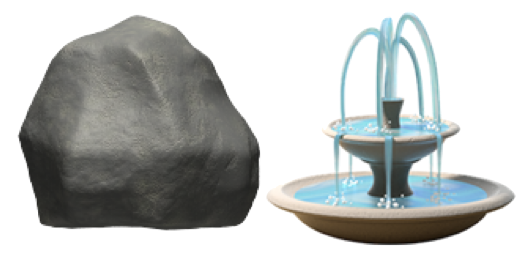
\includegraphics[scale=0.07]{figs/emojis/mini_3.png} & 0 & Hazard Awareness and Equipment Utilization \\
\hline
\rowcolor{gray!10} 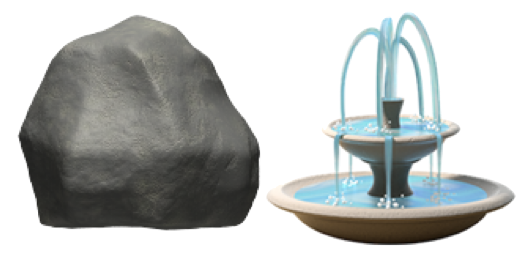
\includegraphics[scale=0.07]{figs/emojis/mini_4.png} & 0 & Boulder Manipulation Strategy \\
\hline
\rowcolor{gray!10} 
\includegraphics[scale=0.07]{figs/emojis/mini_5.png} & 0 & Combat Engagement and Survival \\
\hline
\rowcolor{gray!10} 
\includegraphics[scale=0.07]{figs/emojis/mini_6.png} & 0 & Role-Specific Ability Utilization  \\
\hline
\rowcolor{gray!30} 
\includegraphics[scale=0.07]{figs/emojis/mini_7.png} & 1 & Spatial Awareness and Interpretation  \\
\hline
\rowcolor{gray!30} 
\includegraphics[scale=0.07]{figs/emojis/mini_8.png} & 1 & Object Pickup Efficiency \\
\hline
\rowcolor{gray!60} \includegraphics[scale=0.07]{figs/emojis/mini_9.png} & 2 & Giant Rats Encounter Handling \\
\hline
\end{tabular}
\caption{Metrics and Turn of Introduction for MiniHack}
\label{tab:metrics_mini}
\end{table}

\label{tab:metrics_mini}

\subsubsection{Results}

f

\paragraph{\textit{4.4.3.1 Results}}~\newline 
\\GPT-40-241120 is used as the agent model.
\paragraph{\textit{4.4.3.1 Results}}~\newline 
\\GPT-40-241120 is used as the agent model.

\subsubsection{Results}

f

